% !TeX root = ../main.tex
% Add the above to each chapter to make compiling the PDF easier in some editors.
\chapter{Design and Implementation}\label{chapter:design}

\section{Technology Stack}
In order to implement the architecture proposed in chapter \ref{chapter:method} we choose Android as end user device platform. Android has the highest market share \cite{android-market-share} among mobile devices and offers a healthy ecosystem of frameworks and libraries that simplify development. Furthermore we opted for an implementation in Kotlin instead of Java to reduce boilerplate code and improve readability.

As server side technology we choose node.js in conjunction with a mongoDB object store database. A NoSQL database like mongoDB provides flexibility and easy adaption of data schemes without much overhead and thus perfectly fits our prototyping purpose. We choose node.js out of the same reasons. In contrast to a statically typed language, javascript provides more flexibility and ease of change. Furthermore, node.js is often used in combination with mongoDB and provides seamingless integration.

The results can be made available to the public either via a dedicated route of the server or directly through granting access to the respective collection\footnote{A collection in an object store is the equivalent to a table in an SQL database.} of the database.

The following sections describe the implementation of the Android application and the server and explain design decisions. We start with an outline of the API shared by both, the Android application and the server.\\

\begin{samepage}
\section{API}\label{api}
The API is designed as a pure REST API based on JSON and consists of the following endpoints:
\begin{itemize}
	\item POST /user HTTP/1.1
  \\for creating a new user (see figure \ref{post-user-request} and \ref{post-user-response}).

	\item GET /requests?pk=... HTTP/1.1
  \\for retrieving aggregation requests for a user (see figure \ref{get-requests-response}).

	\item POST /forward HTTP/1.1
  \\for sending a processed aggregation request back to the server (see figure \ref{post-request}).

	\item GET /aggregations HTTP/1.1
  \\for retrieving all completed aggregation results (see figure \ref{get-aggregations}).

	\item POST /admin/sampleRequest HTTP/1.1
  \\for starting a new aggregation request (see figure \ref{insert-sample}).
\end{itemize}
\end{samepage}

\begin{figure}[!h]
  \begin{lstlisting}[language=json,firstnumber=1]
  {
    "publicKey": "-----BEGIN PUBLIC KEY-----\nMIIBIjANBgkqhkiG..."
  }
  \end{lstlisting}
  \caption{POST /user}
  \label{post-user-request}
\end{figure}

\begin{figure}[h!]
  \begin{lstlisting}[language=json,firstnumber=1]
  {
    "publicKey": "-----BEGIN PUBLIC KEY-----\nMIIBIjANBgkqhkiG...",
    "password": "LSFDfzduSFSozfwf"
  }
  \end{lstlisting}
  \caption{Response to POST /user}
  \label{post-user-response}
\end{figure}

\begin{figure}[h!]
  \begin{lstlisting}[language=json,firstnumber=1]
  [{
    "publicKey": "-----BEGIN PUBLIC KEY-----\nMIIBIjANBgkqhkiG...",
    "serverId": "5cfbd6734e733a0079ee5c0f",
    "nextuser" : "-----BEGIN PUBLIC KEY-----\nMIIBIjANBgkqhBms...",
    "encryptionKey":"HXporX7tqrgkf6Cp8OlqOcpLb...",
    "iv":"pMxQ2nHqbz1Zu24Lfi5HYQ==",
    "encryptedRequest":"xtgP2e9AeAK8hfPXQe03..."
  }]
  \end{lstlisting}
  \caption{Response to GET /requests}
  \label{get-requests-response}
\end{figure}

\begin{figure}[h!]
  \begin{lstlisting}[language=json,firstnumber=1]
  {
    "publicKey": "-----BEGIN PUBLIC KEY-----\nMIIBIjANBgkqhkiG...",
    "password": "LSFDfzduSFSozfwf",
    "serverId": "5cfbd6734e733a0079ee5c0f",
    "encryptionKey":"HXporX7tqrgkf6Cp8OlqOcpLb...",
    "iv":"pMxQ2nHqbz1Zu24Lfi5HYQ==",
    "encryptedRequest":"xtgP2e9AeAK8hfPXQe03..."
  }
  \end{lstlisting}
  \caption{POSt /forward}
  \label{post-request}
\end{figure}

\begin{figure}[h!]
  \begin{lstlisting}[language=json,firstnumber=1]
  [{
    "timestamp": 1559216514521,
    "startedAt": 1559216514685,
    "start": "2019-05-28",
    "end": "2019-05-31",
    "type": "steps",
    "n": 6,
    "value": 4271,
    "valueList": []
  },
  {
    "timestamp": 1559216514521,
    "startedAt": 1559216514685,
    "start": "2019-05-28",
    "end": "2019-05-31",
    "type": "stepsListing",
    "n": 5,
    "value": 0,
    "valueList": [1661, 1246, 3195, 7714, 7842]
   }]
  \end{lstlisting}
  \caption{Response to GET /aggregations}
  \label{get-aggregations}
\end{figure}

\begin{figure}[h!]
  \begin{lstlisting}[language=json,firstnumber=1]
  [{
    "password": "adminPassword",
    "start": "2019-05-31",
    "end": "2019-06-05",
    "type": "activity_2",
  }]
  \end{lstlisting}
  \caption{POST /admin/insertDample}
  \label{insert-sample}
\end{figure}

%TODO: Password should go into header in the future.

The routes used for interaction with the application (except the one for creating a new user are secured and can only be used if the user can successfully be authenticated. The routes for starting new aggregation requests and retrieving all results require administrator authentication. The route for the results is designed to be available to the public without authentication. Nevertheless we restrict access only to result types that have been examined to fully protect users' privacy. So, for example, our experimental trajectory request type is not available to the public.

The encryptedRequest field e.g. in figure \ref{get-requests-response} contains the encrypted version of the request described in chapter \ref{chapter:method}.

%//TODO: Integrate this section somewhere else (in methodology)
\subsection{Data Aggregation Design}
All aggregations proposed in section \ref{aggregation-schemes} can be implemented using only 4 fields: An Integer \textit{n} specifying the current number of participants, a Floating Point Number \textit{value} e.g. containing the current mean value of the aggregation, a list \textit{valueList} of Floating Point Numbers that can be reused for different purposes accross requests and a String \textit{type} that specifies the request and the used scheme how the other fields are populated e.g. the encoding of the \textit{valueList}. In addition, all aggregation requests have a start day and an end day. Days' time is always treated as 00:00 o'clock. Thus, the timespan for an aggregation is always a multiple of 24 hours.\\

\begin{samepage}
Due to limited scope of this thesis, only the following out of the aggregation requests defined in section \ref{aggregation-schemes} were implemented:
\begin{enumerate}
	\item Computing the average number of steps walked across all users participating in the request.
	\item Computing the average time spent walking, running, in a vehicle or on a bicycle\footnote{https://developers.google.com/android/reference/com/google/android/gms/location/DetectedActivity}.
	\item Collecting a list of the average number of steps walked by each participant during the timespan.
	\item collecting a list of all trajectories registered by the users' phones.
\end{enumerate}
\end{samepage}

All aggregations work as a prove of concept of the proposed setup and hence serve answering research question 1. Aggregation 1, 2 and furthermore help to investigate which types of aggregations are possible to be published and allow for an investigation whether overlapping timeperiods allow for inference attacks. Thus  they help to answer research question 2 and 3. Aggregation 3 was implemented especially in order to test research question 2.
%whether this type of aggregation, which allows for more advances statistical computations as median values and distribution properties, still completely preserves privacy.
Aggregation 4 imposes a privacy risk discussed in \parencite{twitter, cellphone, krumm} on the user and was implemented in order to get an overview of the data quality of our setup and validate the feasability of the other aggregation requests proposed in section \ref{aggregation-schemes}.

\section{Android Application}
The Android application targets Android Oreo (API level 27) and requires a minimum API level of 19. Approximately 96.8\% of devices run on this or a higher version of Android \cite{android-api-level-share} which allows our application to be installed on the majority of Android devices.
Furthermore, the application leverages Goolge Play Services to obtain GPS and activity data. Without Google Play Services installed, the application will not work. In order to ease future adaptability, we chose to use the Dagger2\footnote{https://dagger.dev/} framework for dependency injection in order to decouple classes as far as possible. Further use of frameworks and libraries will be explained in the following respective sections.

Th application is aimed to collect GPS data, detect the user's current activity and count the user's steps. The data collection process happens in the background without any user interaction needed. Aggregation requests to aggregate data accross devices are also served without any user interaction needed.
\begin{samepage}
The android application can be grouped into three main parts of loosely coupled modules:
\begin{itemize}
	\item A module responsible for collecting and saving raw data
	\item A module responsible for locally aggregating raw data
	\item A module responsible for communicating with the server and handling aggregation requests
\end{itemize}
\end{samepage}

\begin{figure}[h!]
  \caption{Android architecture}
  \label{android-overview}
  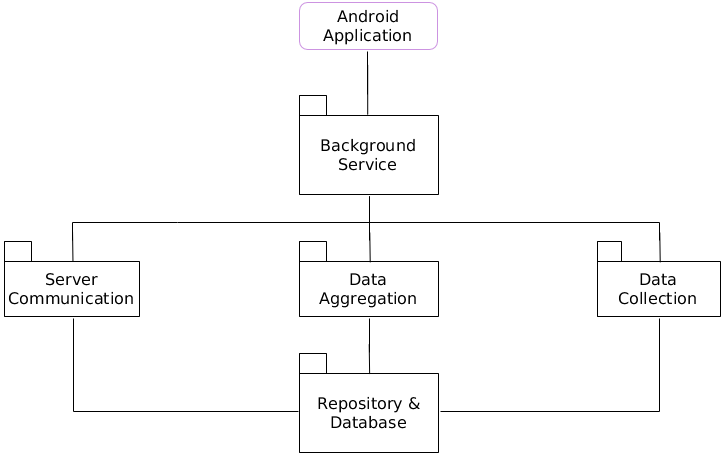
\includegraphics[width=\textwidth]{data/diagrams/android-architecture.png}
\end{figure}

The control flow as depicted in figure \ref{android-overview} is as follows: 
The application has only one Main Activity in order to ask the user to allow location access and start the background services. Apart from that the only Activity does not serve any specific purpose. 
The local aggregation as well as the polling of new requests from the server happens in the background on a 15 minute interval. The Android Workmanager controls this periodic work without any user interaction being required.

For the App in order to have maximum possibilities collecting esspecially GPS data and preventing the Android operating system from shutting down when not interacted with by the user (which is usually never the case), a non-dismissible status notification is displayed at all time\footnote{Compare to the non-dismissible status notification displayed by Google Maps when the navigation system is active}. Also the application is registered to be automatically restarted upon boot\footnote{From Android 6.0 on (API level 23), restricts apps' behaviour in order to reduce battery consumption. E.g. all apps are automatically managed by the battery manager which restricts background launches. The user has to switch this option to manual management in order to allow the app to function in the way it was designed. See https://developer.android.com/guide/background/ and also https://developer.android.com/training/monitoring-device-state/doze-standby} and also when the application is closed by the user (e.g. via the task manager) so that once installed, no further user interaction is necessary.
Furthermore, the application, respectively each module is heavily unit tested in order to guarantee functionality and facilitate further development by other research teams. Unit and integration tests are based on AndroidJUnit4\footnote{See https://developer.android.com/reference/android/support/test/runner/AndroidJUnit4} and the expresso\footnote{See https://developer.android.com/training/testing/espresso} framework.

\subsection{Separation of concerns regarding Data Collection and Aggregation}
We choose to separate the aggregation and collection of location data in order to decouple the modules and provide the possibility to extend the model of aggregated data in the future without the need to change the raw data model. Vice versa the data collection process can be modified without impacting the aggregation process.

\subsection {Data Collection}
We use the Android Room Persistence library\footnote{See https://developer.android.com/topic/libraries/architecture/room} to locally store data. The library provides a layer over the standard LiteSQL database commonly used in many Android applications. We collect three types of data:
\begin{itemize}
	\item Steps: If available, the phone's internal step sensor provides updates on a regular basis. The step sensor always informs about the total number of steps since the last reboot. Upon each time we receive data from the step sensor, this data is stored directly in the \textit{step\_counter\_table}.
	\item User's activities: The Google Play Services  activity recognition API leverages different data and sensors available on the phone in order to inform about the most probable current activity of the user as one of \textit{still, walking, running, in a vehicle, on bicycle}. Whenever there is a change detected, two events are fired - one for exiting the former and one for entering the current activity. The events might not be dispatched instantly but contain the timestamp of the exact occurence. Upon each received event, this data is stored directly in the \textit{activity\_transition\_table}.
	\item GPS positions: GPS data is retrieved through the \textit{FusedLocationProviderClient} which leverages cellphone-tower and WIFI data apart from GPS to determine the position. In order to limit battery consumption, GPS data is only requested every minute if the device's detected activity is \textit{still}\footnote{Neertheless, if other applications request a GPS position, our application also receives this data, even if it occurs on a faster interval}. If the current detected activity is \textit{walking}, the interval is set to 5 seconds and in any other state, the interval is set to every second. The data is stored in the linked tables \textit{gps\_data\_table} and \textit{gps\_location\_table}. We choosse to separate the GPS point itself from the timestamp having in mind that future aggregations might need or leverage the separation of spatial data and time and more than one event might be attached to the same GPS point.
\end{itemize}

\subsection{Local Data Aggregation}\label{local-data-aggregation}
From the received values of the step counter since last reboot saved in \textit{step\_counter\_table} the daily steps are computed and stored in \textit{steps\_table}. The exit and enter events received via the activity recognition framework and stored in the \textit{activity\_transition\_table} are matched in order to compute activities with start and duration. Those activities are then saved in the \textit{activity\_table}.
GPS data is used to compute trajectories through the following algorithm:
\begin{enumerate}
	\item When there are more than 10 minutes between two subsequent GPS points in the sequence of all GPS points to be processed, the sequence is separated into two separate sequences and each is processed separately as a possible trajectory in the next step.
	\item First, we identify still moments - periods of no movement - as follows:
	\begin{enumerate}
		\item For each GPS point, we identify a subsequent GPS point that was registered at least two minutes after the first one.
		\item If the average speed between those two points was below 0.6 m/s, the pair is added to a list to be processed in the next step.
		\item The list of pairs of GPS points resulting from the last step is fused into sequences of GPS points as long as possible: Whenever two pairs overlap in their timestamp, they are fused to a new pair covering the combined timespan.
	\end{enumerate}
	\item The resultig GPS pairs of still moments are used to exclude still moments from the original sequence and divide it into subsequences marking trajectories.
\end{enumerate}
Of each trajectory, the start and end location as well as the respective timestamp are then saved in \textit{trajectory\_table}. We tested 0.5 m/s, 0.6 m/s and 0.7 m/s as threshold in step 2b) and found 0.6 m/s to be best fit the tested sample. On the one hand the threshold must be low enough to still include slow walking which might be below 1 m/s. On the other hand, the threshold should not be too low because inaccuracy in GPS data might otherwise induce trajectories where the device has actually not moved at all.

Example of algorithm (TODO):
\begin{verbatim}
{
	Original dataset:			
	Latitude Longitude Time
	44		 11		   10:11:03
	44.5	 11.1	   10:11:15
	44.4	 11.05	   10:12:12
	44.3	 11.07	   10:33:00
	44	     11.2	   10:34:00
}
\end{verbatim}

\subsection{Serving Aggregation Requests}
We use the retrofit2 framework\footnote{https://square.github.io/retrofit/} based on OKHTTP\footnote{https://square.github.io/okhttp/} to handle communication with our REST server dexribed in \ref{server}. An HTTP Interceptor is used to modify incoming and outgoing requests. The interceptor decrypts the request body of incoming messages using the private key of the installation before the body is parsed into Java Objects. On outgoing messages the inteerceptor adds authentication before sending them to the server.
The app polls for new aggregation requests every 15 minutes. New aggregation requests are first stored locally in the database. Those requests are then processed and the results are again stored locally as pending outgoing requests until they are finally send to the server. Figure XX illustrates this process. This separation of concerns is useful especially in case of an interrupted communication during processing the aggregation request. When the results cannnot be send to the server, the app automatically retries the next time that the communication module is invoked.
The aggregation itself takes the type parameter of the request to specify which actions to take on the three fields (n:int, value:Float, valueList: List<Float>) shared across all aggregation requests. In case of the tyes "steps" and "activity\_X" the field value contains the current mean of the data and the field n is the number of participants so far. In case of "stepsListing" only the field "valueList" is used. Each user's mean value is added to the list. In case of "trajectories", only the field "valueList" is used. Four subsequent elements of the list always represent one trajectory as of latitude of start, longitude of start, latitude of end and longitude of end.

In case that the aggregation should be changed to actually work over P2P e.g. using local WIFI networks this module only has to be adapted to the new routing of requests. No further changes to the application are necessary.
%In case of edge-computing, ... only this module has to be adapted to receive the requets from and send them to the respective endpoints and the system works fine.

\begin{figure}[h!]
  \caption{Server architecture}
  \label{server-architecture}
  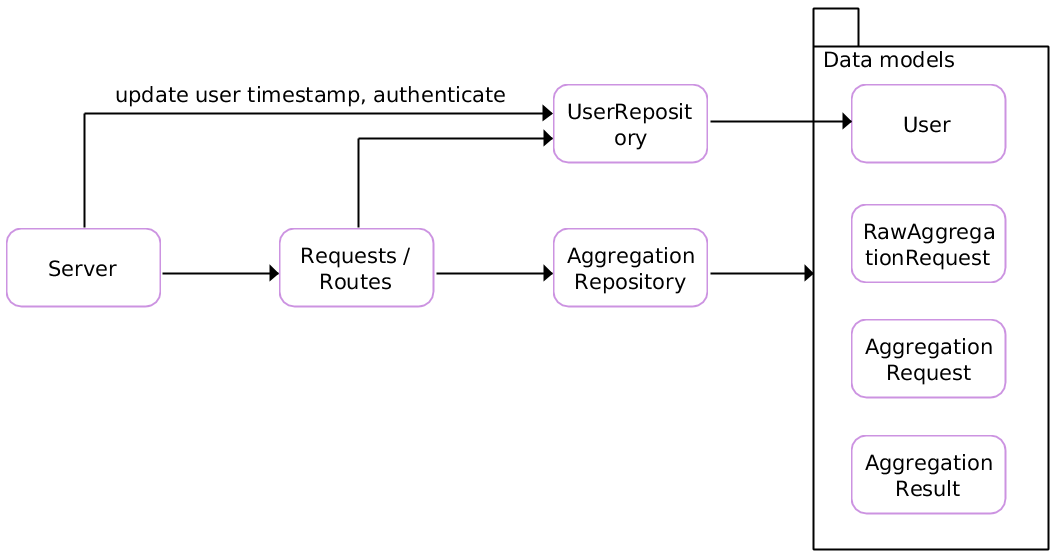
\includegraphics[width=\textwidth]{data/diagrams/server-diagram.png}
\end{figure}

\section{Server Design and Implementation}\label{server}
The server is build using the event-driven node.js verion 10.15.3 leveraging the express\footnote{See https://expressjs.com/} web-server framework and using the mocha\footnote{See https://mochajs.org/} testing framework in combination with the chai\footnote{See https://www.chaijs.com/} assertion library for unit and integration testing. The server is designed using a layered architecture as described in figure \ref{server-architecture}. On the lowest level are the data models which define and verify the data schemes defined in subsection \ref{server-data-model}. The \textit{commonRepository} and the \textit{userRepository} are build on top of those models and persists data in a mongoDB object store. They also handle e.g. transactions where several objects are modified depending on the result of the previous modification (TODO: implement transactions?). The third level provides the logic to be executed for each endpoint defined in \textit{routs.js} while \textit{server.js} on the top level starts the server on the port specified in TODO.environment.json-TODO. It also registers the routes described in section \ref{api}, adds authentication and interacts directly with the \textit{userRepository} in order to update the respective users lastSeen property. Furthermore, it starts a scheduled repeating task to keep the request chain running. This process is described in subsection \ref{request-chain}

\subsection{Data Model}\label{server-data-model}
We organize the data in four collections. The user collection stores the user data which is the public key, the hashed password and "lastSeen" - the timestamp of the last interaction of the user with the server. Aggregation requests are split into two collections. The collection "rawAggregationRequests" stores the initial aggregation request inserted through the admin interface containing the fields start, end, type - the type of the request, the three fields n, value, valueList reused across all aggregations to pass data, the timestamp when the request was filed to the server and a flag indicating whether this request has been started yet\footnote{E.g. when the end data of a newly inserted aggregation request is in the future, the request will be started only when this day has passed}. Upon start of the aggregation request, a list of the 10 most recently active users is retrieved in order to serve this request. The request body is then encrypted with the first users public key and stored in the collection "aggregationRequests". Each time, a user requests an aggregationRequest, proceeds with it and sends the results back to the server, the result is inserted into the database as a new aggregationRequest. The fields of this collection are 
\begin{itemize}
	\item rawRequestId - The id of the related rawRequest. This field is not available through the API.
	\item started\_at - The timestamp, when the request has been started
	\item publicKey - The public key of the user that should proceed this request
	\item nextUser - The public key of the user that will receive the request afterwards. This is necessary so that the user that should proceed this request can encrypt the processed request with the public key of the next user.
	\item previousRequest - The id of the previous request. This is null, if it is the first request in the chain. This is used for the mechanism taking care if a request is not processed by the user it is pending for.
	\item users - the list of public keys of the following users that will proceed with this request. This field is not available through the API.
	\item encryptionKey - A synchronous key, encrypted with the public key of the user the request is aimed at.
	\item iv - the initialization vector used for synchronous encryption and decryption of the actual aggregation request.
	\item encryptedRequest - The actual aggregation request encrypted with the synchronous key.
	\item timestamp - The timestamp when this object has been created.
	\item commpleted - A flag indicating whether this aggregation request has already been proceeded by the respective user and the resulting aggregationRequest has been received by the server.
\end{itemize}
The last collection called "aggregationResults" is used to store the results of an aggregation request. Once there are no more users to serve an aggregationRequest, the last user sends the final data unencrypted to the server where it is stored as an aggregationResult. It contains the same fields as the rawAggregationRequest except the started flag and additionally a field started\_at and timestamp - indicating when the aggregation request referenced through rawRequestId was started and when it was completed.

\subsection{request-chain}\label{request-chain}
//TODO
server.js also invokes a scheduled task which re-routes stale requests where the user has not proceeded with the pending request either due to being offline or due to a problem handling the request. When new aggregation requests are started, the lastSeen timestamp of users is taken into account to exclude users that have not connected for a certain time. Furthermore, the list of users who are selected to serve the new request is ordered by the time the user was last seen.